\documentclass[crop,tikz]{standalone}

\usepackage{makecell}

\definecolor{alizarin}{rgb}{0.82, 0.1, 0.26}
\definecolor{airforceblue}{rgb}{0.36, 0.54, 0.66}
\definecolor{apricot}{rgb}{0.98, 0.81, 0.69}
\definecolor{blush}{rgb}{0.87, 0.36, 0.51}
\definecolor{cadmiumgreen}{rgb}{0.0, 0.42, 0.24}
\definecolor{cambridgeblue}{rgb}{0.64, 0.76, 0.68}
\definecolor{celadon}{rgb}{0.67, 0.88, 0.69}
\definecolor{chestnut}{rgb}{0.8, 0.36, 0.36}
\definecolor{harvardcrimson}{rgb}{0.79, 0.0, 0.09}
\definecolor{darkseagreen}{rgb}{0.56, 0.74, 0.56}
\definecolor{aoenglish}{rgb}{0.0, 0.5, 0.0}
\definecolor{brightube}{rgb}{0.82, 0.62, 0.91}
\definecolor{amethyst}{rgb}{0.6, 0.4, 0.8}
\definecolor{asparagus}{rgb}{0.53, 0.66, 0.42}

\usetikzlibrary{positioning}
\usetikzlibrary{matrix}
\usetikzlibrary{fit}
\usetikzlibrary{calc,decorations.pathmorphing,patterns}
\usetikzlibrary{decorations.pathreplacing}


\newcommand{\vvector}[1]{\tikz{\draw[#1,step=1em,fill=#1!50] (0,0)  grid (1em,4em) rectangle (0, 0);}}
\newcommand{\hvector}[1]{\tikz{\draw[#1,step=1em,fill=#1!50] (0,0)  grid (4em,1em) rectangle (0, 0);}}
\newcommand{\vvectorSmall}[1]{\tikz{\draw[#1,step=.5em,fill=#1!50] (0,0)  grid (.5em,1.5em) rectangle (0, 0);}}

\newdimen\XCoord
\newdimen\YCoord
\newdimen\XXCoord
\newdimen\YYCoord

\newdimen\empty
\newdimen\fromX
\newdimen\fromY
\newdimen\toX
\newdimen\toY

\newcommand{\outgoing}[2]{
  \path (#1); \pgfgetlastxy{\XCoord}{\YCoord};
  \path (#2); \pgfgetlastxy{\XXCoord}{\YYCoord};
  \draw[->, line width=1pt] (\XCoord, \YCoord) -- (\XCoord, \YYCoord);
}%
\newcommand{\incoming}[2]{
  \path (#1); \pgfgetlastxy{\XCoord}{\YCoord};
  \path (#2); \pgfgetlastxy{\XXCoord}{\YYCoord};
  \draw[->, line width=1pt] (\XCoord, \YYCoord) -- (\XCoord, \YCoord);
}%
% horizontal arrow: (#1.x, #3.y) -- (#2.x, #3.y)
\newcommand{\horizontalArrow}[3]{
  \path (#1); \pgfgetlastxy{\fromX}{\empty};
  \path (#2); \pgfgetlastxy{\toX}{\empty};
  \path (#3); \pgfgetlastxy{\empty}{\fromY};
  \draw[->, line width=1pt] (\fromX, \fromY) -- (\toX, \fromY);
}%
% vertical braces: (#3.x, #1.y) -- (#3.x, #2.y)
\newcommand{\verticalBraces}[4]{
  \path (#1); \pgfgetlastxy{\empty}{\fromY};
  \path (#2); \pgfgetlastxy{\empty}{\toY};
  \path (#3); \pgfgetlastxy{\fromX}{\empty};
  % XXX the values for positionning the node for #4 have been choosen for the NMT example. must be checked
  \draw [decorate,decoration={brace,amplitude=3pt,raise=4pt},yshift=0pt] (\fromX, \fromY) -- (\fromX, \toY) node [midway, anchor=west, xshift=.2cm] {#4};
}%


%\newcommand{\plotColor}{airforceblue}
\newcommand{\plotColor}{gray}

\begin{document}


    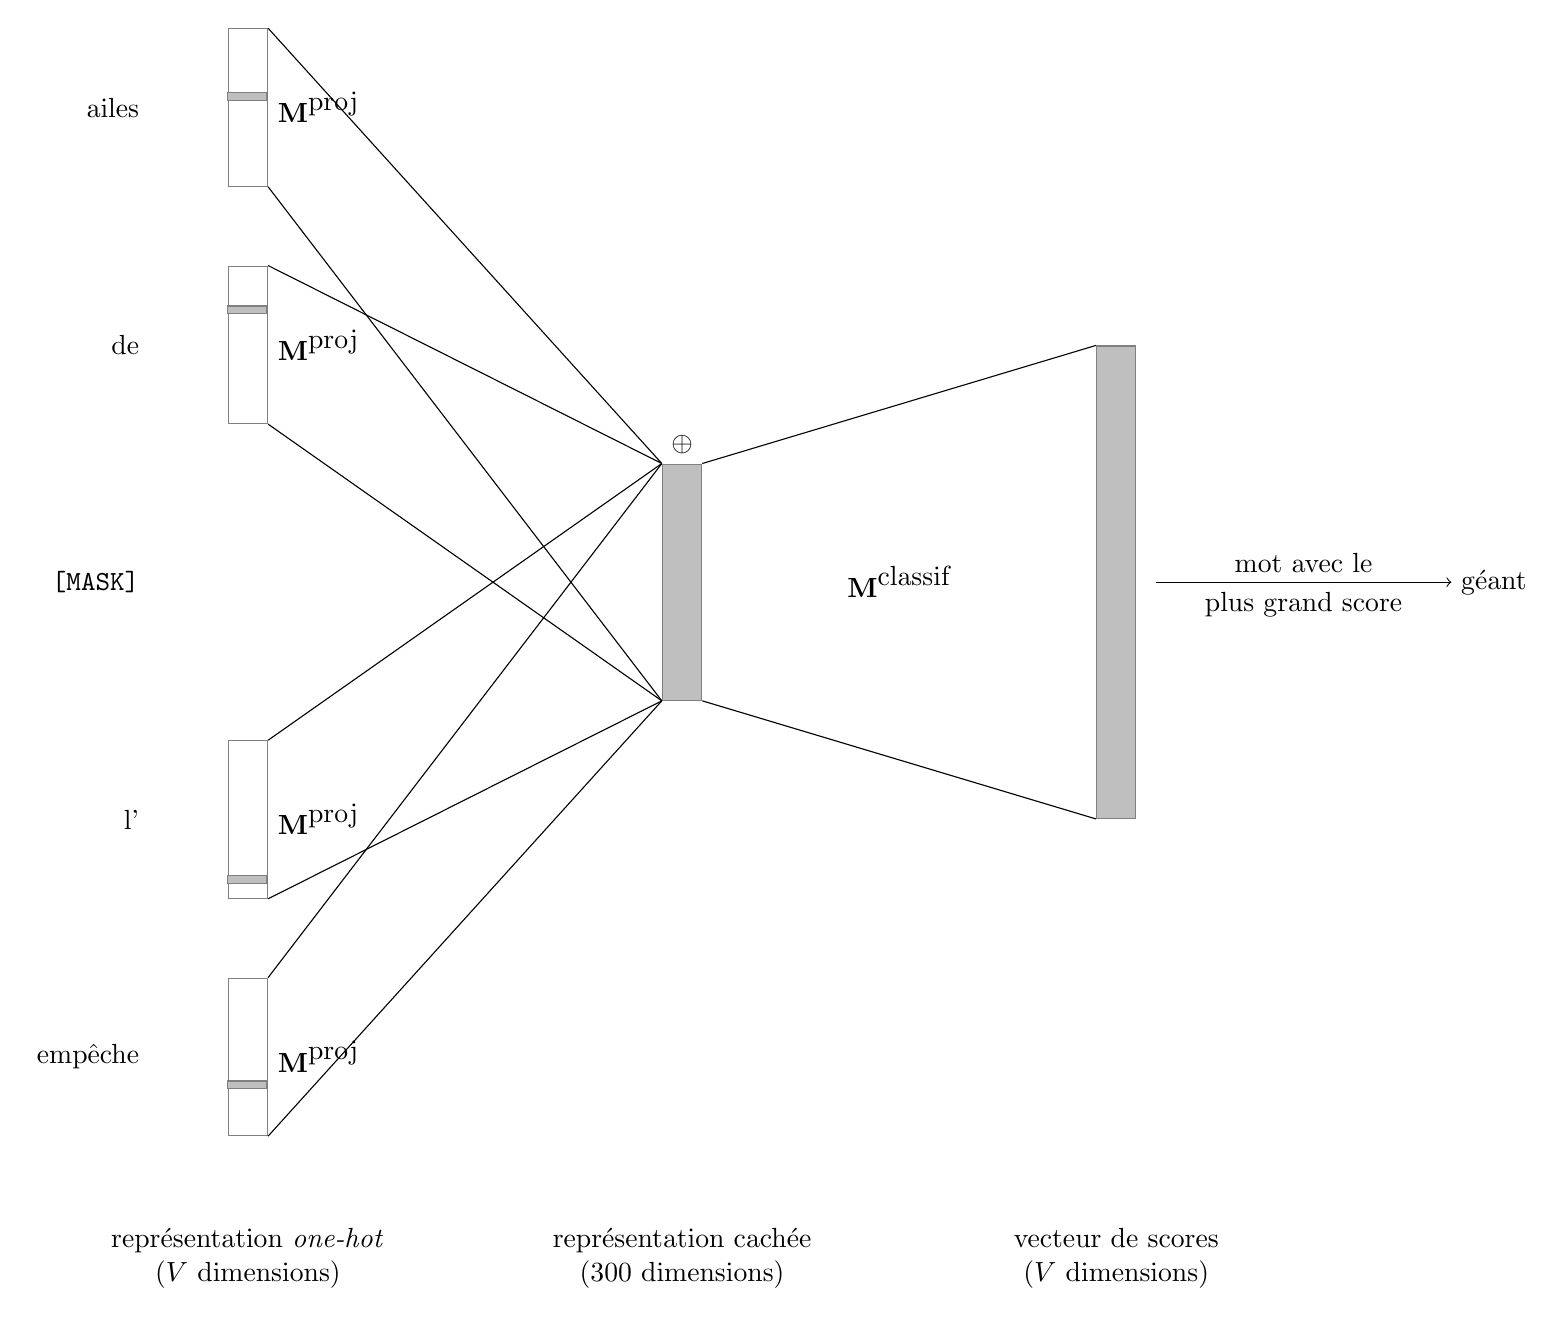
\begin{tikzpicture}
        \pgfmathsetmacro{\onehotsize}{2}      % size of the one hot vector

        \node[draw=\plotColor, minimum width=.5cm, minimum height=\onehotsize{}cm] (w1) at (0cm,0cm) {};
        \node[left=of w1] {ailes};
        \pgfmathsetmacro{\pos}{55} % \pos en pourcentage
        \draw[\plotColor, fill=\plotColor!50] (w1.south west) ++(0, \pos/100*\onehotsize) rectangle ++(0.5, 0.1);


        \node[draw=\plotColor, minimum width=.5cm, minimum height=\onehotsize{}cm, below=of w1] (w2) {};
        \node[left=of w2] {de};
        \pgfmathsetmacro{\pos}{70} % \pos en pourcentage
        \draw[\plotColor, fill=\plotColor!50] (w2.south west) ++(0, \pos/100*\onehotsize) rectangle ++(0.5, 0.1);

        \node[draw=white, minimum width=.5cm, minimum height=\onehotsize{}cm, below=of w2] (w3) {};
        \node[left=of w3] {\texttt{[MASK]}};

        \node[draw=\plotColor, minimum width=.5cm, minimum height=\onehotsize{}cm, below=of w3] (w4) {};
        \node[left=of w4] {l'};
        \pgfmathsetmacro{\pos}{10} % \pos en pourcentage
        \draw[\plotColor, fill=\plotColor!50] (w4.south west) ++(0, \pos/100*\onehotsize) rectangle ++(0.5, 0.1);

        \node[draw=\plotColor, minimum width=.5cm, minimum height=\onehotsize{}cm, below=of w4] (w5) {};
        \node[left=of w5] {empêche};
        \pgfmathsetmacro{\pos}{30} % \pos en pourcentage
        \draw[\plotColor, fill=\plotColor!50] (w5.south west) ++(0, \pos/100*\onehotsize) rectangle ++(0.5, 0.1);

        \node[draw=\plotColor, fill=\plotColor!50, right=of w3, xshift=4cm, minimum height=3cm, minimum width=.5cm] (hidden) {};

        \node[draw=\plotColor, fill=\plotColor!50, right=of hidden, xshift=4cm, minimum height=6cm, minimum width=.5cm] (score) {};

        \draw (w1.north east) -- (hidden.north west);
        \draw (w1.south east) -- (hidden.south west);

        \draw (w2.north east) -- (hidden.north west);
        \draw (w2.south east) -- (hidden.south west);

        \draw (w4.north east) -- (hidden.north west);
        \draw (w4.south east) -- (hidden.south west);

        \draw (w5.north east) -- (hidden.north west);
        \draw (w5.south east) -- (hidden.south west);
      
        \draw (hidden.north east) -- (score.north west);
        \draw (hidden.south east) -- (score.south west);

        \draw[draw=white] (hidden) -- (score) node[baseline=mid,pos=.5] {$\textbf{M}^{\textrm{classif}}$};

        \node [right=4cm of score] (pred) {géant};

        \draw[->] (score) ++(.5cm, 0) -- (pred) node [pos=.5, below] {plus grand score} node [pos=.5, above] {mot avec le};

        \node[right=of w1, xshift=-1cm] {$\textbf{M}^{\textrm{proj}}$};
        \node[right=of w2, xshift=-1cm] {$\textbf{M}^{\textrm{proj}}$};
        \node[right=of w4, xshift=-1cm] {$\textbf{M}^{\textrm{proj}}$};
        \node[right=of w5, xshift=-1cm] {$\textbf{M}^{\textrm{proj}}$};

        \draw node [above=0cm of hidden] {$\oplus$};

        \draw node [below=of w5] (label1) {\makecell{représentation \textit{one-hot} \\ ($V$~dimensions)}};

        \node (C) at (label1 -| hidden) {\makecell{représentation cachée \\ (300~dimensions)}};

        \node (C) at (label1 -| score) {\makecell{vecteur de scores \\ ($V$~dimensions)}};

    \end{tikzpicture}
\end{document}